\documentclass[tikz, border=4pt]{standalone}
\usepackage{tikz}
\begin{document}
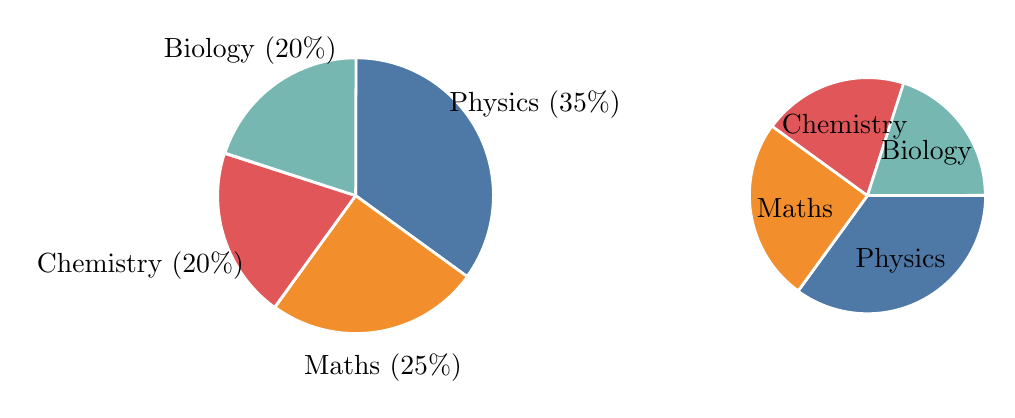
\begin{tikzpicture}[x=1cm, y=1cm]
  \definecolor{tdc1}{HTML}{4E79A7}
  \definecolor{tdc2}{HTML}{F28E2B}
  \definecolor{tdc3}{HTML}{E15759}
  \definecolor{tdc4}{HTML}{76B7B2}

  \fill[tdc1, draw=white, line width=1pt, line join=round] (0,0) -- (0,1.75) arc[start angle=90, end angle=-36, radius=1.75] -- cycle;
  \fill[tdc2, draw=white, line width=1pt, line join=round] (0,0) -- (1.42,-1.03) arc[start angle=-36, end angle=-126, radius=1.75] -- cycle;
  \fill[tdc3, draw=white, line width=1pt, line join=round] (0,0) -- (-1.03,-1.42) arc[start angle=-126, end angle=-198, radius=1.75] -- cycle;
  \fill[tdc4, draw=white, line width=1pt, line join=round] (0,0) -- (-1.66,0.54) arc[start angle=-198, end angle=-270, radius=1.75] -- cycle;
  \node[anchor=207] at (1.69,0.86) {Physics (35\%)};
  \node[anchor=99] at (0.3,-1.88) {Maths (25\%)};
  \node[anchor=18] at (-1.81,-0.59) {Chemistry (20\%)};
  \node[anchor=-54] at (-1.12,1.54) {Biology (20\%)};
  \fill[tdc1, draw=white, line width=1pt, line join=round] (6.5,0) -- (8,0) arc[start angle=0, end angle=-126, radius=1.5] -- cycle;
  \fill[tdc2, draw=white, line width=1pt, line join=round] (6.5,0) -- (5.62,-1.21) arc[start angle=-126, end angle=-216, radius=1.5] -- cycle;
  \fill[tdc3, draw=white, line width=1pt, line join=round] (6.5,0) -- (5.29,0.88) arc[start angle=-216, end angle=-288, radius=1.5] -- cycle;
  \fill[tdc4, draw=white, line width=1pt, line join=round] (6.5,0) -- (6.96,1.43) arc[start angle=-288, end angle=-360, radius=1.5] -- cycle;
  \node at (6.92,-0.83) {Physics};
  \node at (5.58,-0.15) {Maths};
  \node at (6.21,0.88) {Chemistry};
  \node at (7.25,0.55) {Biology};
\end{tikzpicture}
\end{document}
